\chapter{SocioMap}

Aplikace \textbf{SocioMap} je navržena jako interaktivní sociální síť zaměřená na sdílení a objevování událostí prostřednictvím mapového rozhraní. Celý koncept se opírá o rychlost a intuitivní ovládání, které umožňuje uživatelům snadno interagovat s obsahem a ostatními uživateli. Klíčovým prvkem aplikace je právě Google mapa, kde se veškeré události zobrazují jako barevně odlišné markery – každý reprezentuje jednu událost, která se právě na tom místě bude v budoucnu odehrávat. Aplikace poskytuje několik způsobů filtrování, přepínání režimů a vyhledávání.

\section*{Navigace mezi fragmenty}

Navigace v aplikaci probíhá primárně prostřednictvím spodního navigačního panelu označeného jako 'btnNavMenu', který je přístupný z  hlavních částí aplikace. Těmi hlavními částmi aplikace jsou tyto:
\begin{itemize}
	\item \textbf{Mapa (MapFragment)} základní obrazovka aplikace.
	\item \textbf{Profil (ProfileFragment)} sekce s osobními údaji uživatele.
	\item \textbf{Přehled (OverviewFragment)} seznam všech událostí spojené s uživatelem.
\end{itemize}

Přechody mezi fragmenty jsou okamžité, bez zbytečného zdržování, a uživatel tak může aplikaci ovládat velmi intuitivně. Buďto člověk využívá již zmíněné navigační menu mezi hlavními částmi a dále se dostává pomocí tlačítek.
\cite{YouTubeTutorial}


\section{Architektura aplikace}

Architektura aplikace SocioMap je navržena modulárně, aby bylo možné jednotlivé části snadno rozšiřovat. Aplikace je strukturována do logických balíčků (packages) dle odpovědnosti dané komponenty. Tato organizace zajišťuje lepší přehlednost kódu.

Všechny hlavní části aplikace jsou psány v jazyce Java a organizovány podle následující stromové struktury:

\begin{itemize}
  \item \textbf{Admin} – Obsahuje komponenty určené výhradně pro správce systému. Správce má přístup k seznamu uživatelů, může zobrazovat jejich detaily a případně zakazovat přístup nebo je povýšit na status \textit{famous}.
  \begin{itemize}
    \item \texttt{AdminProfile.java} – hlavní rozhraní administrátora.
    \item \texttt{AdminUserList.java} – komponenta pro zobrazování seznamu uživatelů.
    \item \texttt{AdminUserDetails.java} – zobrazuje podrobnosti o vybraném uživateli.
  \end{itemize}

  \item \textbf{Login} – Zajišťuje registraci a přihlášení uživatelů.
  \begin{itemize}
    \item \texttt{Register.java} – aktivita pro registraci nového uživatele, včetně validace a propojení s Firestore.
    \item \texttt{Login.java} – hlavní přihlašovací aktivita, prozatím nepodporuje Google Sign-In.
    \item \texttt{GoogleRegister.java} – slouží k doplnění údajů po přihlášení přes Google účet. Zatím nevyužíván.
  \end{itemize}

  \item \textbf{Main} – Jádro celé aplikace. Obsahuje tři hlavní podsložky podle jednotlivých fragmentů:
  \begin{itemize}
    \item \texttt{MainActivity.java} – základní třída pro správu spodní       navigace a přepínání mezi fragmenty.
    \item \textbf{Map} – součást odpovědná za mapové rozhraní:
    \begin{itemize}
      \item \texttt{MapsFragment.java} – hlavní logika zobrazování markerů, filtrování a interakce s mapou.
      \item \texttt{AddMarkerActivity.java} – přidání nové události kliknutím do mapy.
      \item \texttt{EditMarkerActivity.java} – úprava dříve vytvořené události.
      \item \texttt{MarkerInfoActivity.java} – detailní informace o konkrétní události. Pokud je uživatel vlastník, zobrazují se mu tlačítka na úpravu
    \end{itemize}

    \item \textbf{Profile} – zajišťuje správu osobního účtu:
    \begin{itemize}
      \item \texttt{ProfileFragment.java} – hlavní obrazovka s osobními údaji a možností úprav.
      \item \texttt{EditProfileActivity.java} – umožňuje změnu osobních údajů.
    \end{itemize}

    \item \textbf{Other} – doplňkové části, které nejsou hlavními obrazovkami, ale slouží k rozšíření funkcionality a obecnému přehledu:
    \begin{itemize}
      \item \texttt{OverviewFragment.java} – Přehled všech událostí.
      \item \texttt{FollowingActivity.java} – zobrazuje seznam přátel, které uživatel sleduje.
      \item \texttt{SearchUsersActivity.java} – umožňuje vyhledávat další uživatele.
    \end{itemize}

  \end{itemize}

  \item \textbf{Pomocné třídy} – nachází se mimo výše uvedené složky:
  \begin{itemize}
    \item \texttt{User.java} – modelová třída pro uchování údajů o uživateli.
    \item \texttt{UserListAdapter.java} – adaptér pro zobrazování seznamu uživatelů.
    \item \texttt{EmailSender.java} – pomocná třída pro odesílání emailů (např. při ověření nebo správě účtů).
    \item \texttt{NetworkChangeReceiver.java} – komponenta pro zjišťování a kontrolu dostupnosti připojení k internetu.
  \end{itemize}
\end{itemize}




\newpage
\begin{forest}
  for tree={
    grow=east,   % Strom roste zleva doprava
    parent anchor=east,
    child anchor=west,
    align=center,
    edge={draw, thick},
    font=\ttfamily\scriptsize,  % Zmenšení písma
    s sep=4pt,  % Vertikální mezera
    l sep=6pt   % Horizontální mezera
  }
  [java
    [Admin
        [AdminProfile.java]
        [AdminUserDetails.java]
        [AdminUserList.java]
    ]
    [Login
        [GoogleRegister.java]
        [Login.java]
        [Register.java]
    ]
    [Main
        [Map
            [AddMarkerActivity.java]
            [EditMarkerActivity.java]
            [MarkerInfoActivity.java]
            [MapsFragment.java]
        ]
        [Other
            [OtherFragment.java]
            [FollowingActivity.java]
            [SearchUsersActivity.java]
        ]
        [Profile
            [ProfileFragment.java]
            [EditProfileActivity.java]
        ]
        [MainActivity.java]
    ]
    [EmailSender.java]
    [NetworkChangeReceiver.java]
    [User.java]
    [UserListAdapter.java]
  ]
\end{forest}





\subsection*{Struktura a propojení komponent} \label{sec:structure}

Každá část aplikace je odpovědná za svůj úkol a komunikuje s ostatními komponentami přes zřetelně definovaná rozhraní. Fragmenty jsou spravovány pomocí 'MainActivity', která zajišťuje plynulé přepínání mezi jednotlivými hlavními obrazovkami. Dále se odkazují pomocí tlačítek. 

Aplikace komunikuje s Firebase (Firestore a Authentication) napříč všemi moduly pomocí 'endpointů' – od přihlášení, přes ukládání a načítání uživatelů a událostí, až po správu dat v reálném čase. Přístup k databázi Firebase (konkrétně Firestore) probíhá pomocí oficiálního \texttt{Firebase Java SDK}, které je do projektu přidáno jako závislost pomocí \texttt{build.gradle}. Komunikace s databází je asynchronní – data jsou načítána pomocí\textit{addOnSuccessListener()} nebo \textit{addSnapshotListener()}.

Endpointový dotaz na Firebase:
\begin{figure}[H]
    \centering
    \begin{lstlisting}[language=Java, style=myJavastyle, caption={Endpoint - dotázání se na databázi}]
    firestore.collection("markers")
    .whereGreaterThan("latitude", userLocation.latitude - latOffset)
    .whereLessThan("latitude", userLocation.latitude + latOffset)
    .get()
    .addOnSuccessListener(queryDocumentSnapshots -> {
        if (!queryDocumentSnapshots.isEmpty()) {
            for (DocumentSnapshot document : queryDocumentSnapshots) {
                Double latitude = document.getDouble("latitude");
                Double longitude = document.getDouble("longitude");
                String title = document.getString("title");

                if (latitude != null && longitude != null && title != null) {
                    LatLng markerPosition = new LatLng(latitude, longitude);
                    googleMap.addMarker(new MarkerOptions()
                        .position(markerPosition)
                        .title(title));
                }
            }
        }
    })
    .addOnFailureListener(e -> {
        Log.e("Firestore", "Error - loading markers", e);
    });
    
    \end{lstlisting}
\end{figure}


Data se z Firestore vrací ve formě \textit{DocumentSnapshot}, odkud je lze získat pomocí metod jako \textit{getString()}, \textit{getDouble()} apod.

Mapové rozhraní je realizováno pomocí knihovny \textbf{Google Maps SDK for Android}, která je také přidána do projektu přes \texttt{build.gradle}. Fragment s mapou je definován pomocí \texttt{SupportMapFragment}, který se načítá v rámci 'MapsFragment':

\begin{figure}[H]
    \centering
    \begin{lstlisting}[language=Java, style=myJavastyle, caption={Načítání GoogleMaps Api - \texttt{SupportMapFragment}}]
    SupportMapFragment mapFragment = 
    (SupportMapFragment) getChildFragmentManager()
        .findFragmentById(R.id.map);
    mapFragment.getMapAsync(this);
    \end{lstlisting}
\end{figure}



V metodě \texttt{onMapReady()} pak dochází k práci s objektem \texttt{GoogleMap}, na který se přidávají markery, nastavuje se zoom, lokalizace a další prvky mapy.


Použití pomocných tříd, jako je \texttt{NetworkChangeReceiver}, zajišťuje kontrolu dostupnosti připojení a celkovou robustnost aplikace. 
\cite{JavaDocs} \cite{YouTubeTutorial} \cite{FirebaseDocs} \cite{GoogleMapAPI}  \cite{GoogleMapsAPI}



\section{Logika zobrazování a interakce}

\subsection*{MainActivity.java}

Tato aktivita představuje hlavní vstupní bod aplikace po přihlášení uživatele. Zajišťuje zobrazení spodní navigační lišty a řízení přepínání mezi jednotlivými fragmenty:

\begin{itemize}
    \item \textbf{MapFragment} – zobrazení událostí na mapě,
    \item \textbf{OtherFragment} – přehled přihlášených a vytvořených událostí,
    \item \textbf{ProfileFragment} – uživatelský profil a nastavení.
\end{itemize}

Při kliknutí na jednotlivé položky navigace se načítají odpovídající fragmenty. Aplikace si uchovává aktivní stav, a proto zůstává uživatel v posledním zvoleném okně i při rotaci displeje nebo návratu do aplikace.

Aktivita také načítá data o uživateli a v případě, že se jedná o slavnou osobu, aplikuje speciální design.





\subsection*{MapsFragment}

\begin{figure}[H]
    \centering
    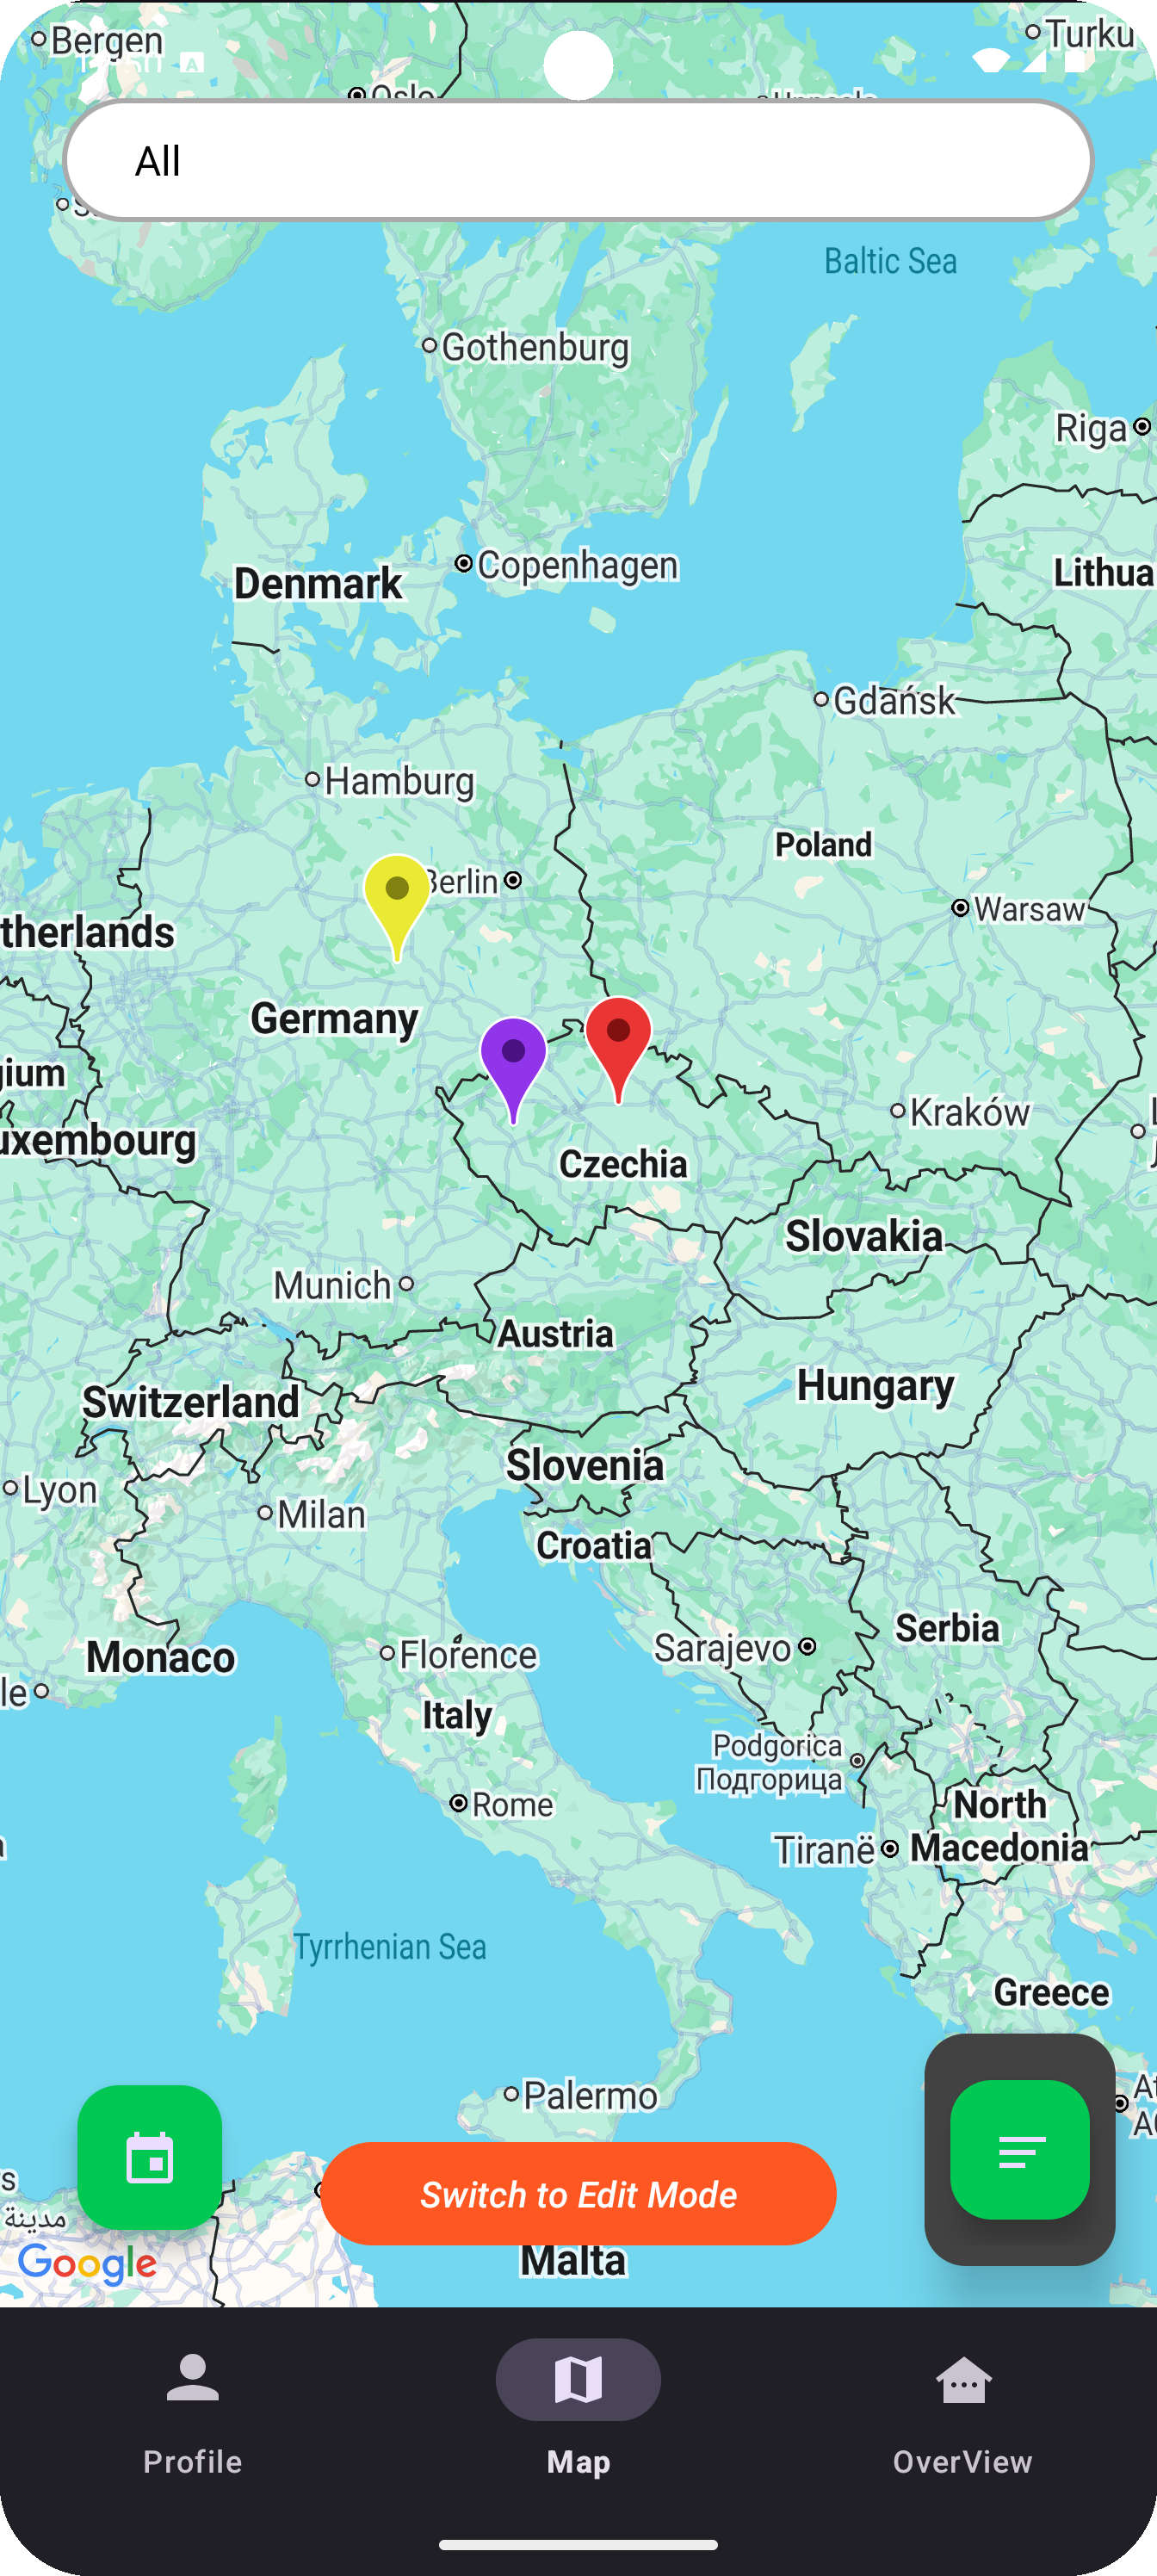
\includegraphics[height=11cm]{Images/MapsFrag.png}
    \caption{MapsFragment}
    \label{fig:Update-account}
\end{figure}

Zobrazování událostí je centralizováno do MapFragmentu. Uživatel se v mapě pohybuje pomocí tahů prstů zoom-in/out. Markery se načítají z databáze Firebase Firestore, kde jsou události uloženy. Každý marker se zobrazuje v jiné barvě podle tematického zaměření události (např. sport, hudba, festival apod.), které může vyfiltrovat. Uživatelská interakce s markery je možná pomocí jednoduchého kliknutí, které otevře okno s názvem a popisem události, a následně může uživatel přejít na detailní obrazovku události.

Součástí mapového rozhraní je filtrovací panel, který lze rozbalit a sbalit. Pomocí něj může uživatel filtrovat pouze události, kterých se účastní přátelé, filtrovat podle tvůrců, které sleduje, nebo zobrazit pouze události pořádané slavnými osobami.


Aplikace bere ohled na nezletilé, tudíž je-li uživatel příliš mladý na danou akci, automaticky se mu událost neukáže. Věkovou hranici nastavuje tvůrce akce. 

Z hlediska režimu ovládání aplikace je možné přepnout do režimu úprav, kdy může uživatel přidat vlastní událost kliknutím na libovolné místo na mapě. Tento režim skrývá všechny filtry, aby nedocházelo k rušení při přidávání nové události.

Na základě uživatelovy polohy dokáže aplikace také zvýraznit „nejlepší událost v okolí“ – pomocí algoritmu, který zohledňuje vzdálenost, oblíbená témata, historii účasti a aktivitu přátel. Lze využít lokalizování a přiblížení uživatele pomocí tlačítka od Googlu v pravém horním rohu. 

Všechny markery, které teprve budou nadcházet, se sesbírají z kolekce 'markers', kde se vezmou pouze jejich koordinace (longitude, latitude) a tématika, kvůli zbarvení.



\begin{figure}[H]
    \centering
\begin{lstlisting}[language=Java, style=myJavaStyle, caption={Metoda \texttt{loadMarkers()} – načítání a filtrování událostí}, label={lst:loadMarkers}]
private void loadMarkers() {
    firestore.collection("users").document(userId).get().addOnSuccessListener
    (userDoc -> {
        int userAge = calculateAge(userDoc.getString("birthyear"));

        firestore.collection("markers").get().addOnSuccessListener(
        queryDocumentSnapshots -> {
            googleMap.clear();
            Date now = new Date();

            for (DocumentSnapshot document : queryDocumentSnapshots) {
                String title = document.getString("title");
                String theme = document.getString("theme");
                String eventDateTime = document.getString("eventDateTime");
                int ageLimit = document.getLong("ageLimit").intValue();

                if (userAge < ageLimit) continue;
                if (!passesAllFilters(document)) continue;

                LatLng position = new LatLng(
                    document.getDouble("latitude"),
                    document.getDouble("longitude")
                );

                googleMap.addMarker(new MarkerOptions()
                    .position(position)
                    .title(title)
                    .icon(BitmapDescriptorFactory.defaultMarker(getMarkerColor(theme)))
                ).setTag(document.getId());
            }
        });
    });
}
\end{lstlisting}
\end{figure}

Tato metoda slouží k načtení všech událostí z databáze a jejich vykreslení na mapě. Před samotným zobrazením se kontroluje věk uživatele vůči minimálnímu věkovému limitu každé události, dále se aplikují filtry (např. podle data, tématu, známých osob nebo přátel), a pokud událost projde těmito podmínkami, je zobrazena na mapě.

\begin{figure}[H]
    \centering
    
\begin{lstlisting}[language=Java, style=myJavaStyle, caption={Změna barvy markeru podle tématu události}, label={lst:marker-colors}]
private float getMarkerColor(String theme) {
    if (theme == null) return BitmapDescriptorFactory.HUE_RED;

    switch (theme.toLowerCase()) {
        case "sports":
            return BitmapDescriptorFactory.HUE_BLUE;
        case "music":
            return BitmapDescriptorFactory.HUE_VIOLET;
        case "festival":
            return BitmapDescriptorFactory.HUE_YELLOW;
        case "workshop":
            return BitmapDescriptorFactory.HUE_GREEN;
        case "custom":
            return BitmapDescriptorFactory.HUE_ORANGE;
        default:
            return BitmapDescriptorFactory.HUE_RED;
    }
}
\end{lstlisting}
\end{figure}



Tato metoda vrací barvu, kterou bude mít marker na mapě podle zadaného tématu události. Pomocí konstrukce \textit{switch} se porovnává textový řetězec tématu a přiřazuje se odpovídající hodnota barvy z \texttt{BitmapDescriptorFactory}. Pokud je téma neznámé nebo chybí, použije se výchozí červená barva.
\cite{FirebaseFirestoreFilter} \cite{GoogleMapAPI}  \cite{GoogleMapsAPI} \cite{AndroidDatePicker}







\subsection*{AddMarkerActivity}

Tato aktivita slouží k přidání nové události na mapu. Uživatel se na tuto obrazovku dostane kliknutím na libovolné místo v mapě v režimu „Úpravy“. V úvodu obrazovky se zobrazí formulář, ve kterém uživatel vyplňuje název události, stručný popis, zvolenou tematiku (např. sport, hudba, festival), věkové omezení a přesný čas konání.

Formulář rovněž obsahuje datumový a časový výběr pomocí příslušných dialogových oken, které zajišťují správné formátování vstupu. Veškeré údaje jsou validovány — např. datum musí být v budoucnosti, některá pole jsou povinná.

Po úspěšném přidání je uživatel automaticky přesměrován zpět do mapového zobrazení, kde se nová událost objeví po synchronizaci jako nový marker. Logika v této aktivitě je tedy zcela propojena s databází a aktuální polohou uživatele.

Nový marker se uloží do kolekce 'markers', kde vznikne pod novým ID. \cite{AndroidDatePicker}





\subsection*{MarkerInfoActivity}

\begin{figure}[H]
    \centering
    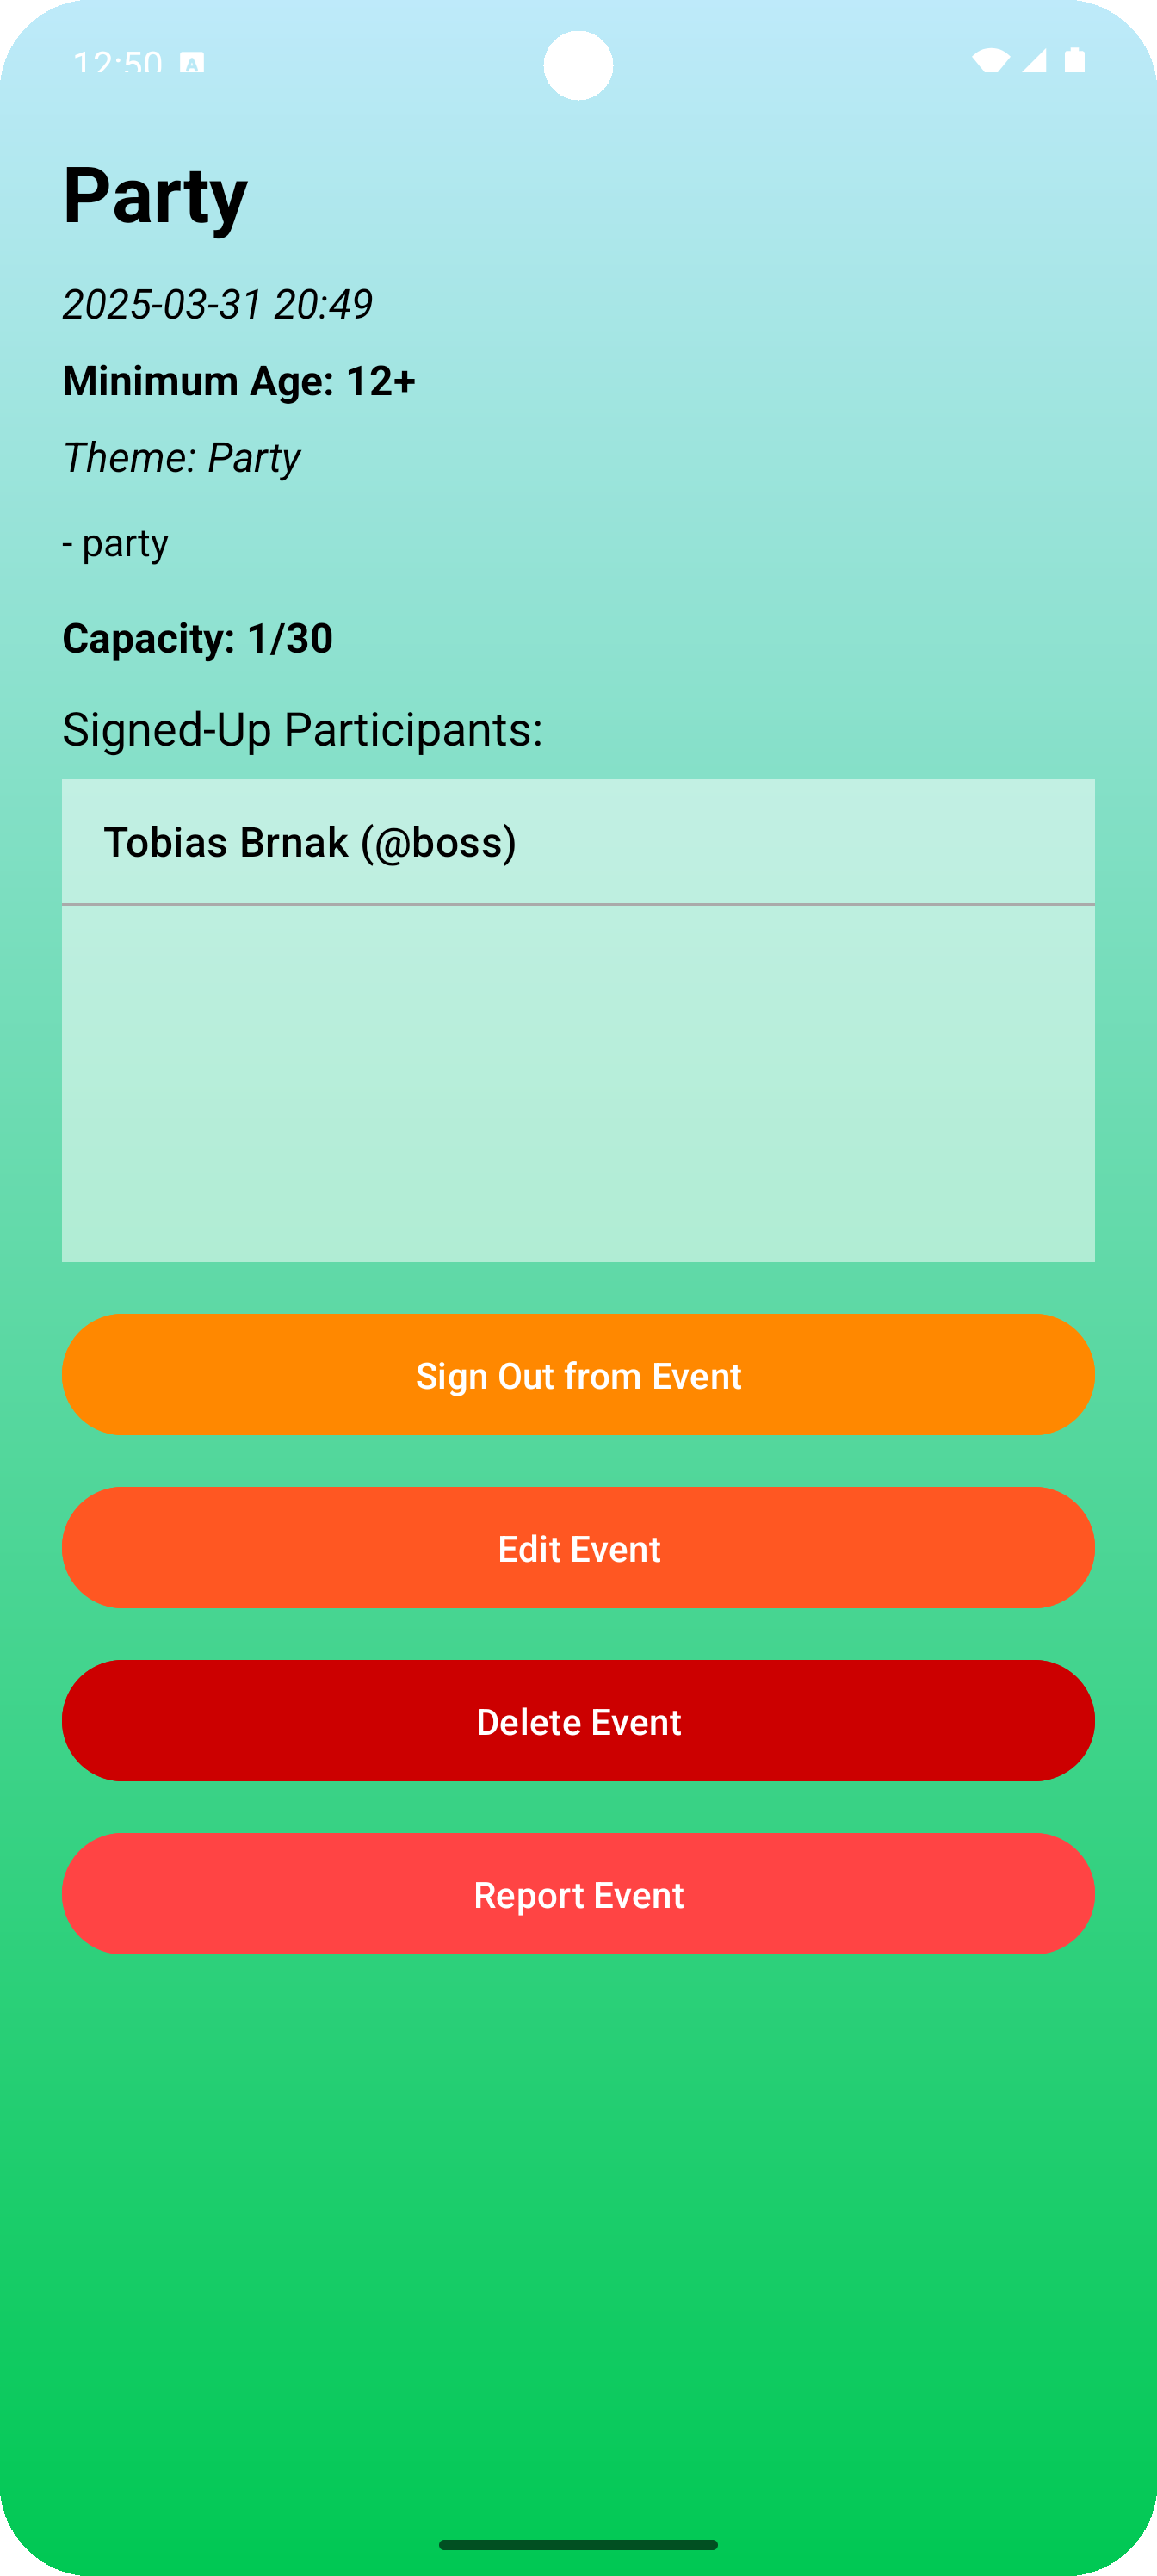
\includegraphics[height=11cm]{Images/MarkerInfo.png}
    \caption{MarkerInfoActivity}
    \label{fig:Update-account}
\end{figure}

Tato aktivita slouží jako detailní přehled konkrétní události, která byla vybrána z mapového zobrazení. Obsahuje všechny dostupné informace o události – název, popis, téma, datum a čas, věkové omezení, pozici na mapě i informace o tvůrci události.

Zobrazí se zde i možnost přihlášení se na danou událost (tlačítko „Zúčastnit se“), pokud se uživatel ještě nezúčastnil, případně možnost odhlášení. Uživatel zde také vidí, kolik dalších lidí se události účastní. Též vidí kolik míst zbývá do plné kapacity události.

Pokud je uživatel tvůrcem události, má navíc k dispozici tlačítko editace (přesměrování do 'EditMarkerActivity') a mazání události.

Získává základní informace z kolekce 'users'. Nadále je vyplní do kolonek a po uložení se použije příkaz aktualizace databáze.

Tato aktivita vyhledá ID markeru v kolekci 'markers' a vypíše všechna informace. Seznam přihlášení se vezme z kolekce 'event\_guest\_list', kde pod stejným ID jsou napsání uživatelé, kteří se na akci přihlásili.






\subsection*{EditMarkerActivity}

Editační aktivita slouží ke správě již existující události, kterou vytvořil sám uživatel. Přístup k této obrazovce je možný skrze detail události `MarkerInfoActivity` pouze v případě, že je aktuálně přihlášený uživatel zároveň tvůrcem dané události.

Zobrazuje předvyplněný formulář s údaji o události, jako je název, popis, datum a čas, tematické zaměření a případné věkové omezení. Uživatel může libovolné pole upravit, a následně změny uložit. Náhled události se po editaci aktualizuje i v mapovém zobrazení.

Tato aktivita rovněž umožňuje zrušit událost úplným smazáním. Bezpečnostní kontrola zajišťuje, že danou událost může upravovat a mazat výhradně její vlastník.

Získává základní informace z kolekce 'markers'. Nadále je vyplní do kolonek a po uložení se použije příkaz aktualizace databáze.





\subsection*{ProfileFragment}

\begin{figure}[H]
    \centering
    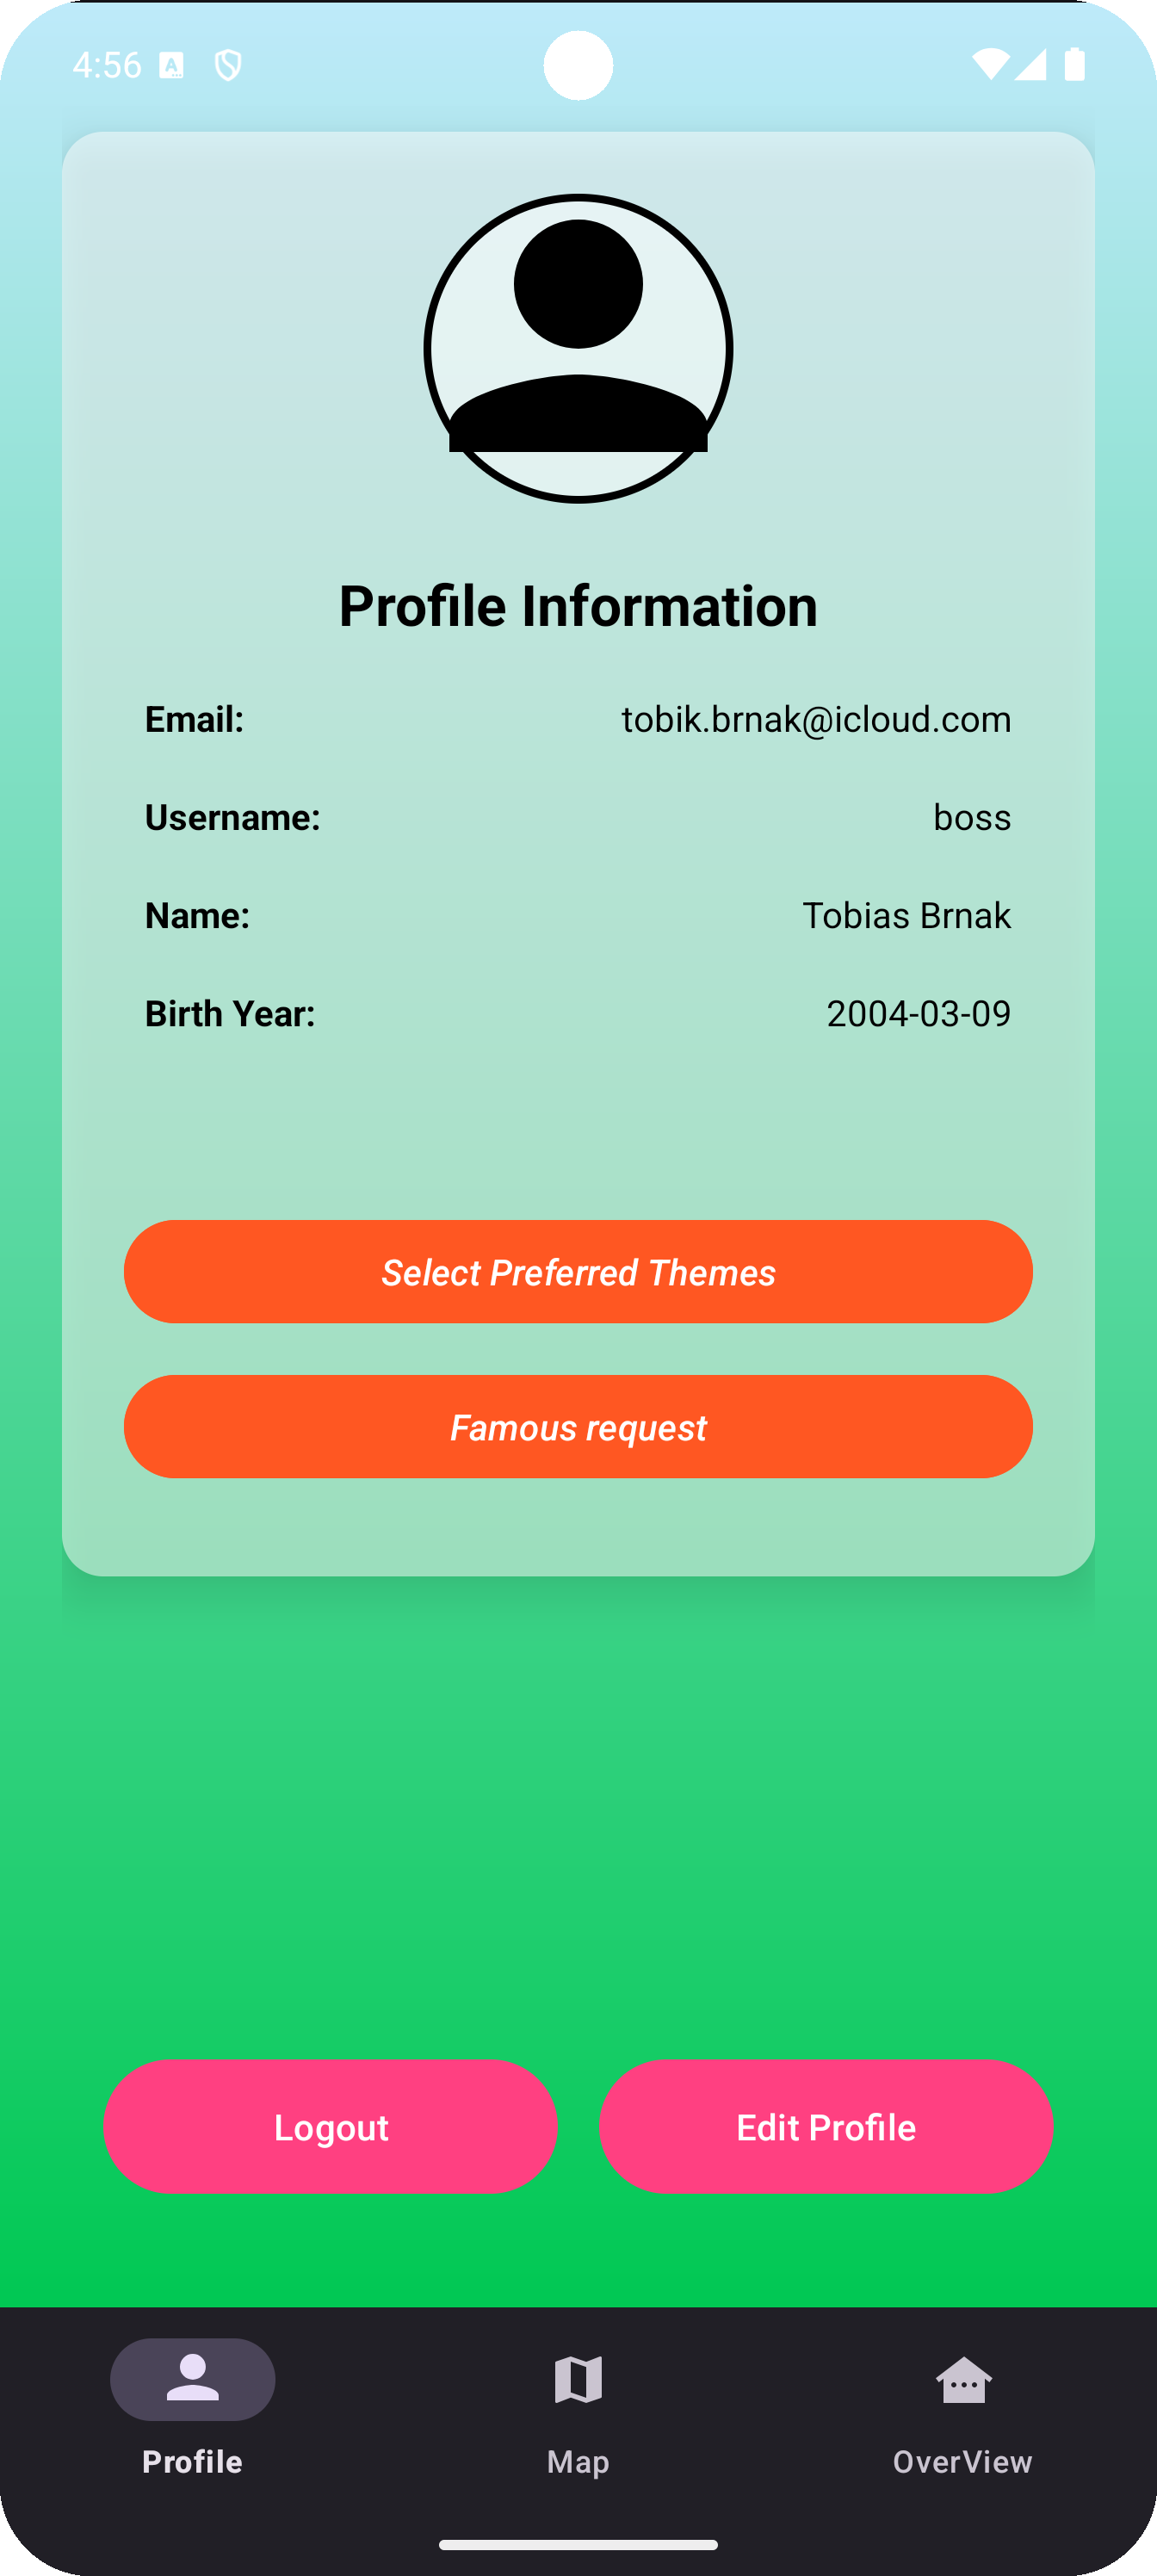
\includegraphics[height=11cm]{Images/Profile_frag.png}
    \caption{ProfileFragment}
    \label{fig:Update-account}
\end{figure}

Tento fragment slouží jako uživatelský profil. Po načtení fragmentu se zobrazí informace přihlášeného uživatele - přezdívka (username), jméno, příjmení, e-mail a rok narození. Tyto informace jsou zobrazeny formou přehledného seznamu v kartičce.

Uživatel má možnost upravit své osobní údaje kliknutím na tlačítko Editovat profil, které ho přesměruje do aktivity 'EditProfileActivity', odhlásit se z aplikace pomocí tlačítka Odhlásit se, které spustí návrat na přihlašovací obrazovku, nebo si vybrat oblíbená témata událostí kliknutím na tlačítko Vybrat témata, což otevře výběrové dialogové okno se seznamem témat.

Pokud je uživatel slavný (\textit{Famous}), je jeho profilový obrázek automaticky změněn na ikonku korunky. Tím je vizuálně odlišena jeho identita.

'ProfileFragment' vyhledá ID shodné s přihlášeným uživatelem a vypíše dané informace, které se následně zobrazí.



\subsection*{EditProfileActivity}

Tato aktivita umožňuje uživateli upravit své základní osobní údaje. Po načtení se automaticky předvyplní stávající data – přezdívka (username), jméno, příjmení a rok narození. 

Uživatelské rozhraní obsahuje vstupní pole pro každou informaci a tlačítko pro potvrzení změn. Při odeslání dat proběhne kontrola platnosti zadaných údajů (např. zda nejsou prázdné) a následně dojde k jejich aktualizaci v dokumentu přihlášeného uživatele.

Získává základní informace z kolekce 'users'. Nadále je vyplní do kolonek a po uložení se použije příkaz aktualizace databáze.



\subsection*{OverviewFragment}

Tento fragment slouží jako přehled účasti uživatele. Uživatel zde najde 4 hlavní sekce seznamů:
\begin{itemize}
    \item Události, které uživatel vytvořil a budou se konat – bere je z kolekce 'markers', kde zjišťuje, zda se schoduje 'userID' s ID přihlášeného uživatele.
    \item Události, na které vytvořil a již se konaly – dotázání se na kolekci 'user\_owner\_arch'
    \item Události, na které se přihlásil v budoucnu – dotázání se na kolekci 'user\_events'
    \item Události, na které se přihlásil v minulosti – dotázání se na kolekci 'user\_arch'

\end{itemize}

Každá událost je zobrazena jako jednoduchý seznam s názvem a datem. Kliknutím na konkrétní událost se uživatel přesměruje do detailu události (`MarkerInfoActivity`), kde si může zobrazit detaily nebo se z události odhlásit.

Tento fragment je vhodný pro rychlou orientaci v historii a plánech uživatele.
\cite{FirebaseFirestoreFilter} 







\subsection*{FollowingActivity}

\begin{figure}[H]
    \centering
    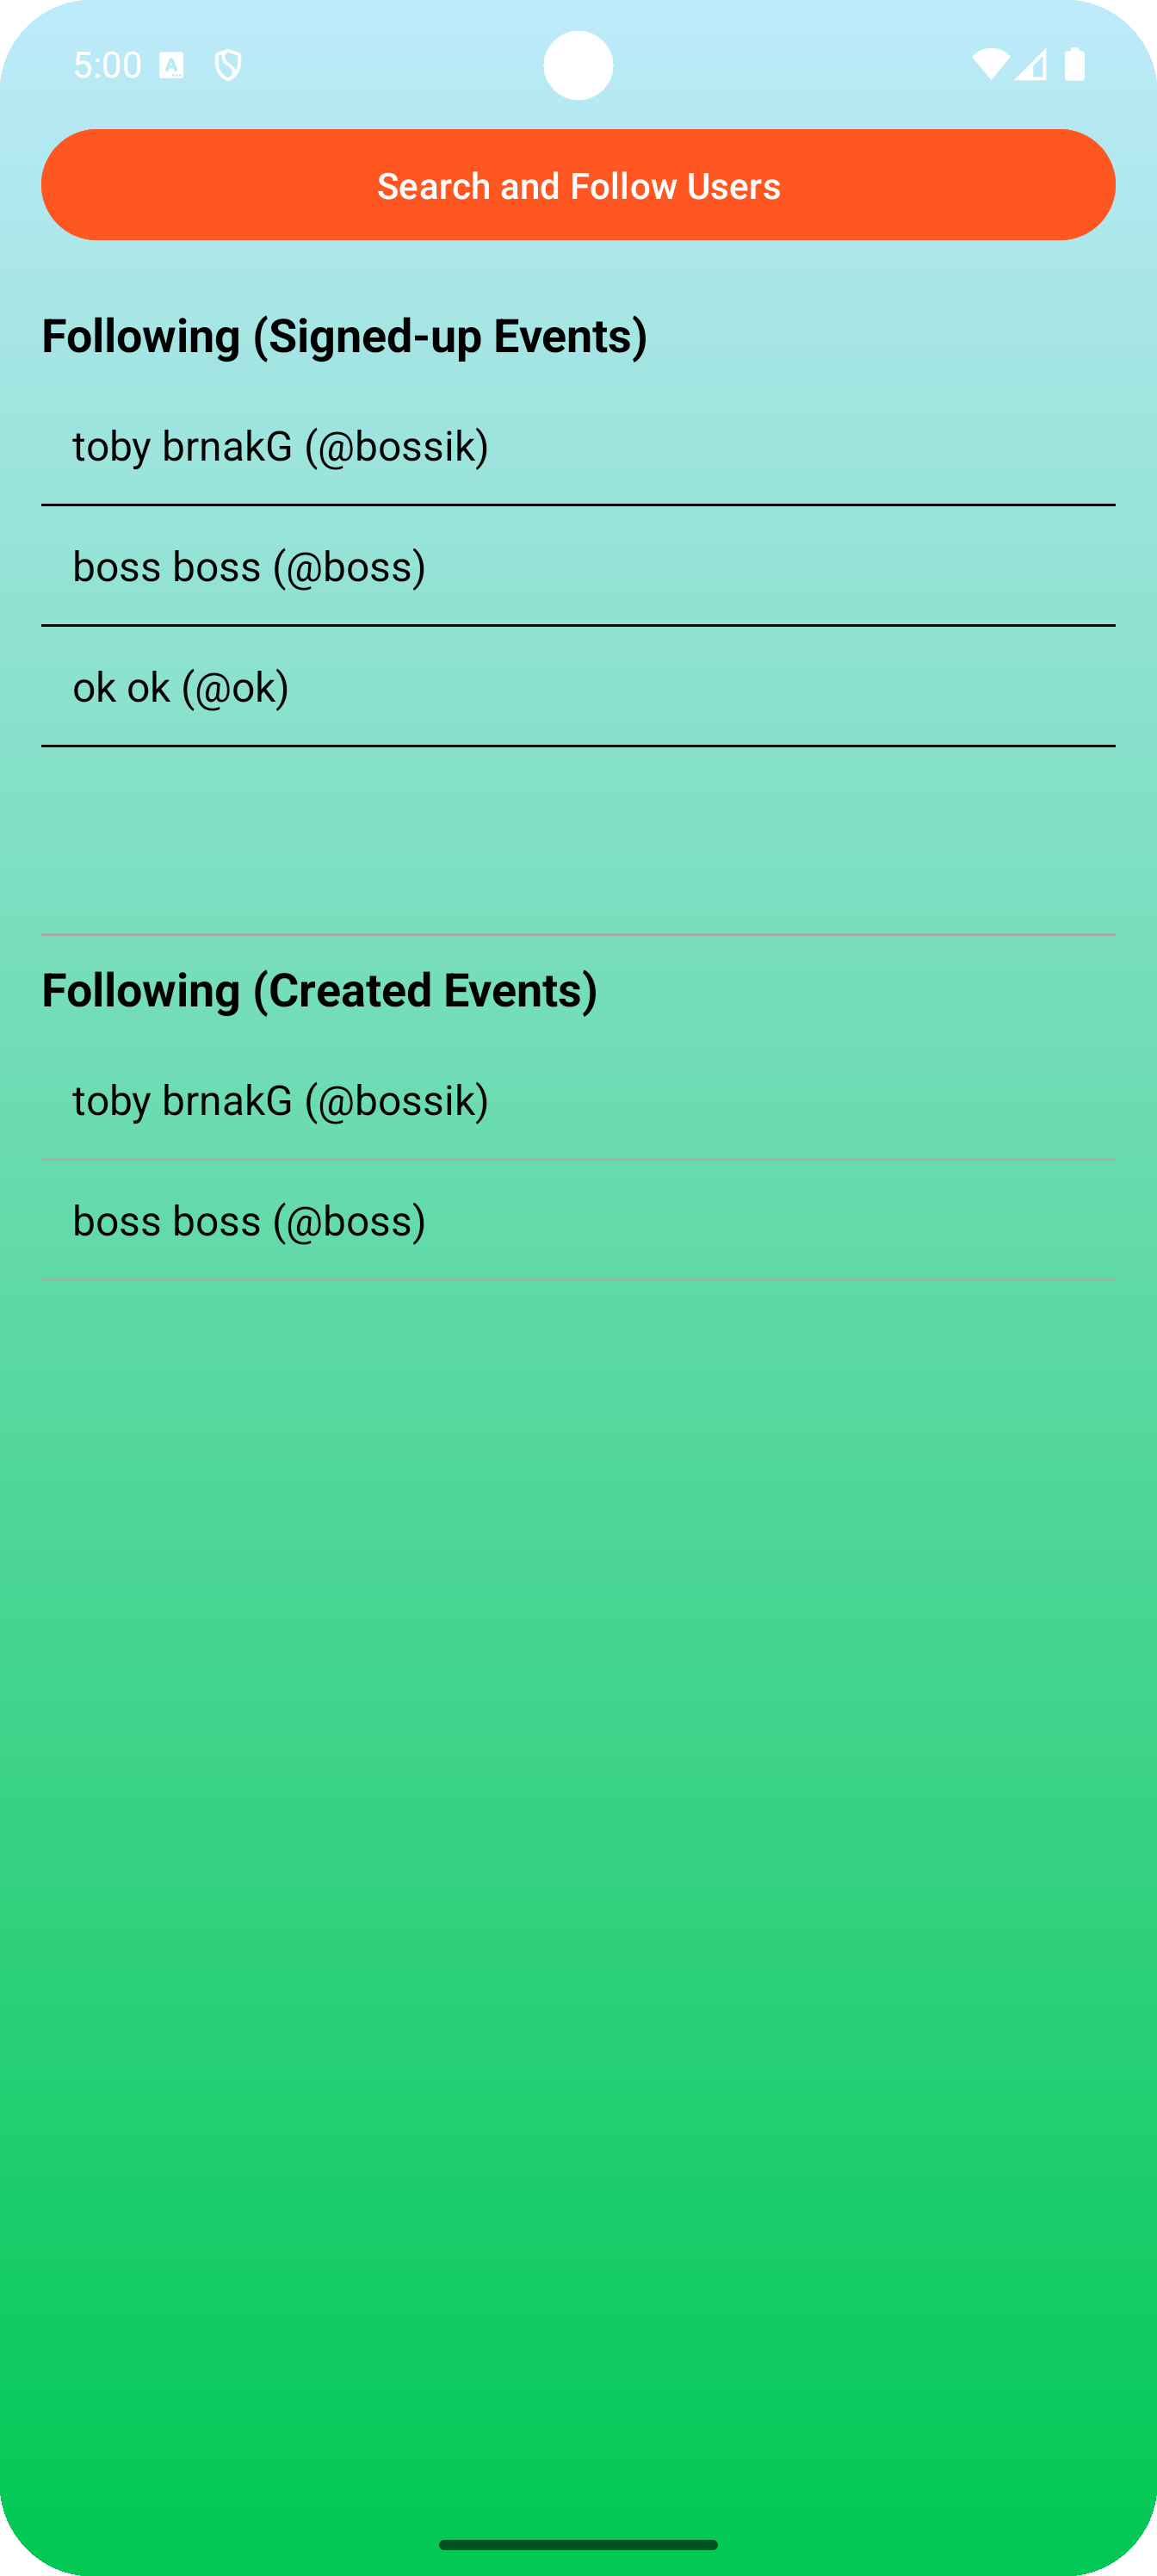
\includegraphics[height=11cm]{Images/Following_activity.png}
    \caption{FollowingActivity}
    \label{fig:Update-account}
\end{figure}

Aktivita umožňuje zobrazit seznam uživatelů, které daný uživatel sleduje, a to jak v roli tvůrců, tak přihlášených přátel. Aktivita je vybavena dvěma seznamy uživatelů. Sbírá data z kolekce 'user\_signup\_follow' a 'user\_create\_follow'







\subsection*{SearchUsersActivity}

\begin{figure}[H]
    \centering
    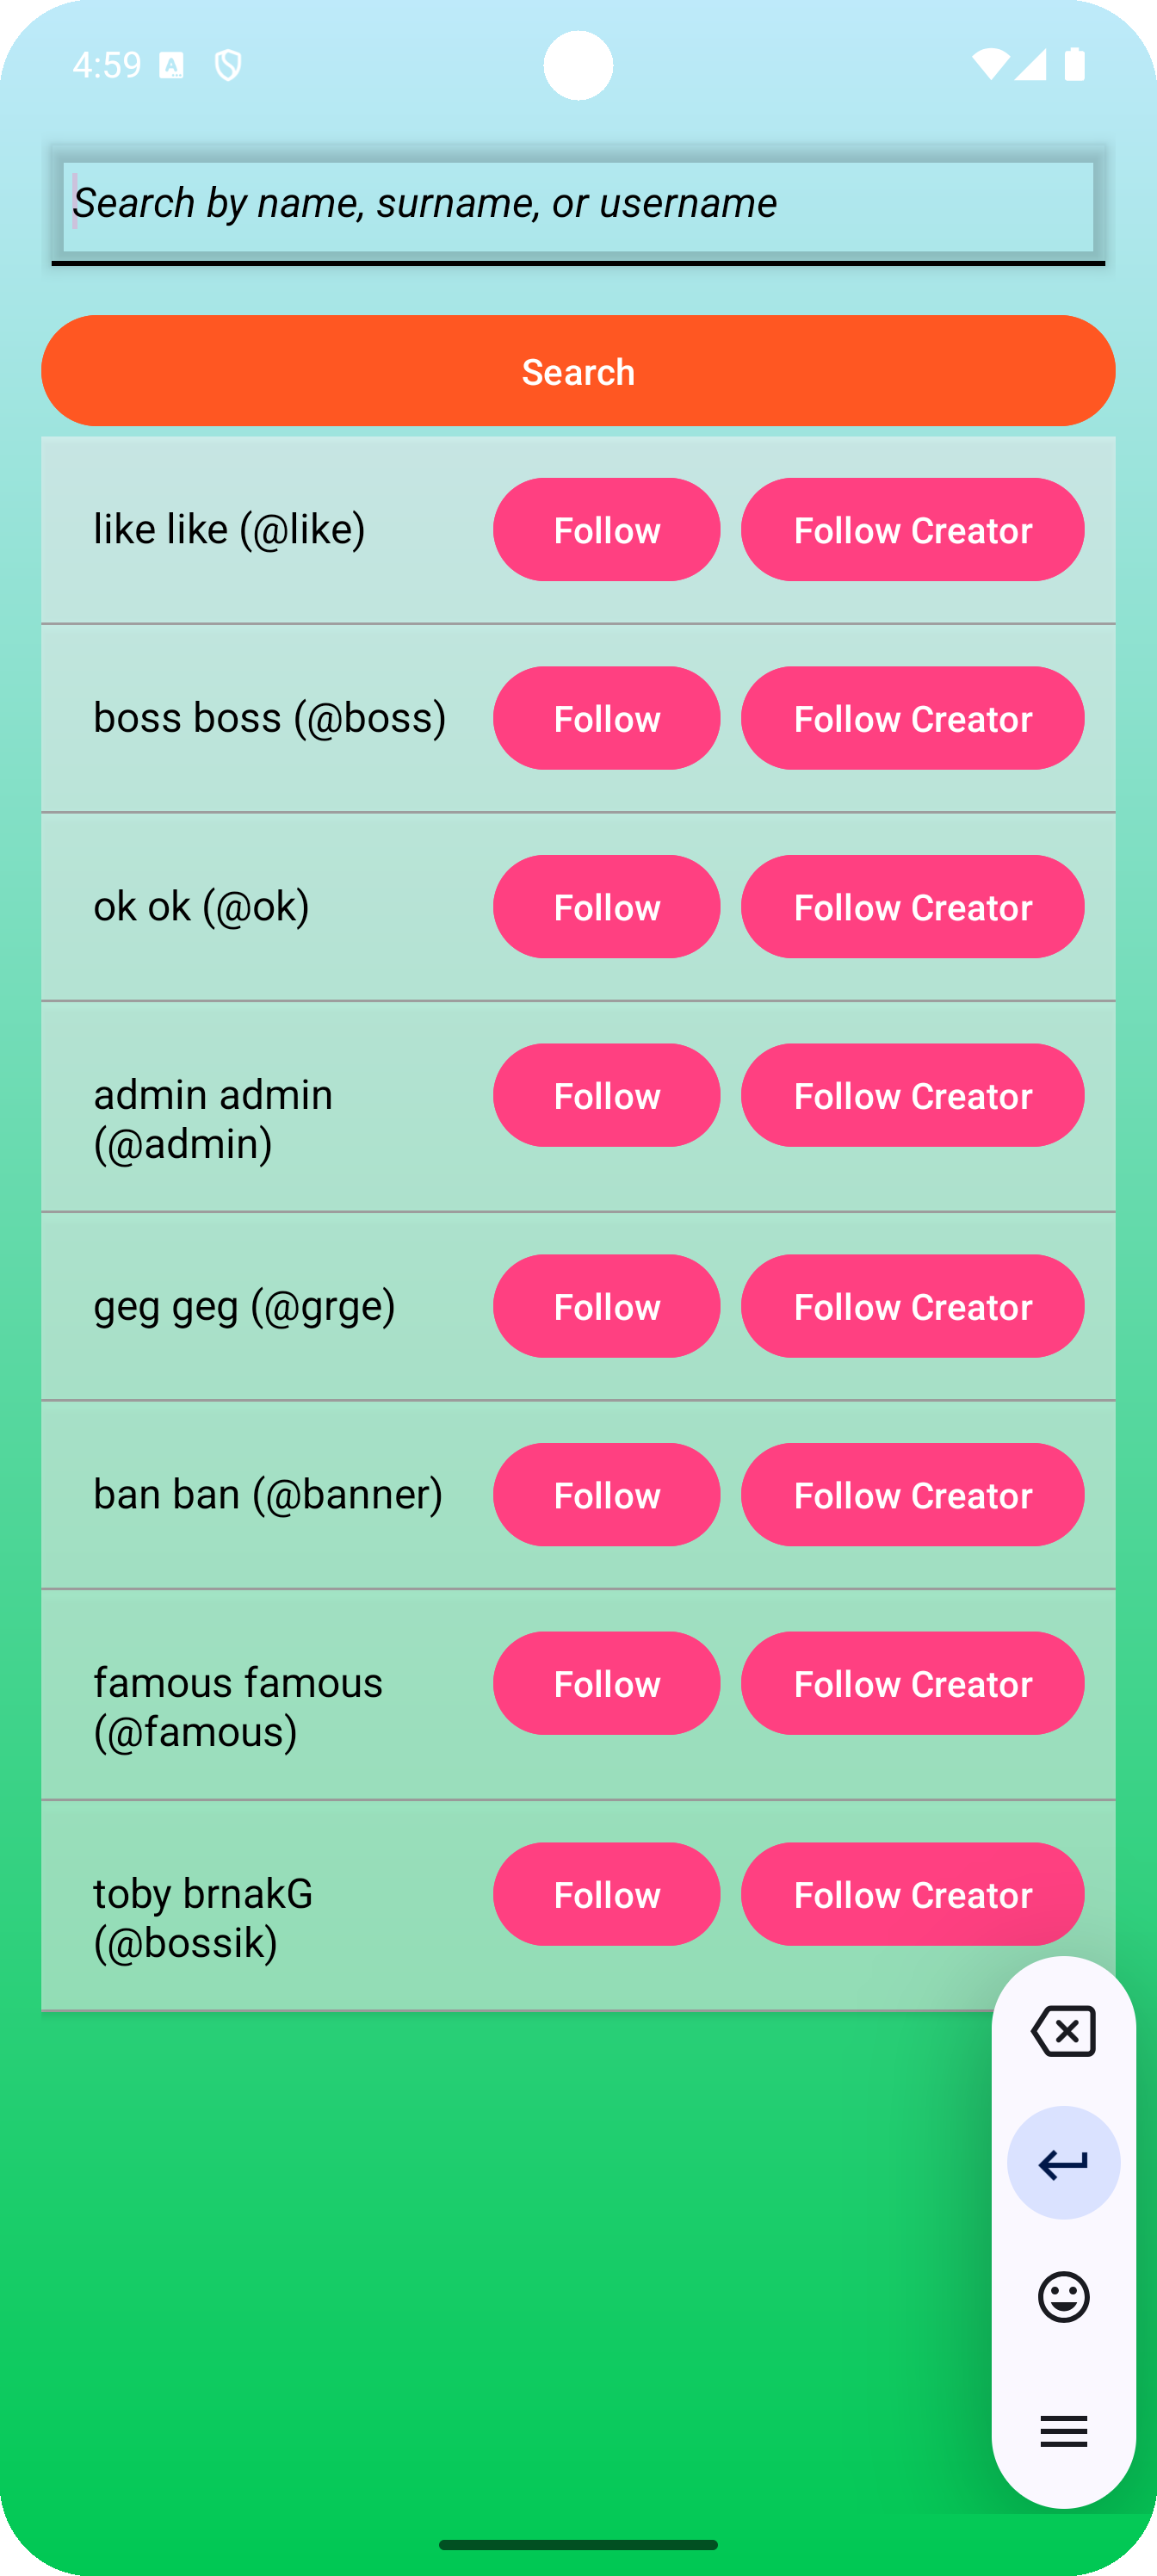
\includegraphics[height=11cm]{Images/Search_users_Following.png}
    \caption{SearchUsersActivity}
    \label{fig:Update-account}
\end{figure}

Tato aktivita slouží k vyhledávání ostatních uživatelů v databázi. Po zadání jména nebo přezdívky se vyfiltrují odpovídající výsledky. U každého uživatele má uživatel možnost zobrazit základní informace, začít sledovat daného uživatele z důvodu, kam se přihlašuje (Follow), nebo začít sledovat daného uživatele z důvodu jeho tvorby (Follow creator).


Načítání uživatelů je pomocí adaptéru ve třídě 'UserAdapter', která dále využívá další třídu 'User' shrnující základní informace o uživateli. Filtrování funguje pomocí dotázání se příkazem \textit{.whereEqualTo()}. Po stisknutí jednoho z tlačítek se informace zapíše do kolekce      'user\_signup\_follow' nebo 'user\_owner\_follow' pod dokument ID přihlášeného uživatele, uživatel, kterého zaklikne, že chce sledovat.
\cite{FirebaseFirestoreFilter}






\subsection*{AdminProfile.java}

Tato aktivita představuje hlavní rozhraní pro administrátora aplikace. Po přihlášení jako administrátor je uživatel přesměrován právě sem. Od této aktivity se administrátor může dostávat do jiných odvětví.

Zde má administrátor možnost kliknout na tlačítko, kde se zobrazí přehled všech uživatelů aplikace 'AdminUserList'a nebo se může z aplikace odhlásit.




\subsection*{AdminUserList.java}

Třída slouží pro získání a zobrazení seznamu všech registrovaných uživatelů aplikace.

Uživatelé jsou zobrazováni v přehledném seznamu. Seznam je interaktivní – kliknutím na položku je administrátor přesměrován na detailní zobrazení konkrétního uživatele.

Součástí je již využitá základní logika filtrování a aktualizace dat. Funguje na stejném principu jako aktivita 'SearchUsersActivity'.









\subsection*{AdminUserDetails.java}

Tato aktivita zobrazí detailní informace o konkrétním uživateli, vybraném z předchozího seznamu. Zobrazuje všechny informace z databáze.


Administrátor zde může pomocí přepínačů měnit atributy uživatele – například přidělit mu roli admina, slavné osoby nebo ho zabanovat. Po úpravách jsou změny ihned synchronizovány s Firestore databází.

Po kliknutí na kartičku se vyhledá v kolekci 'users' id dokumentu shodný s ID uživatelem, na který bylo kliknuto.

\begin{figure}[H]
    \centering
    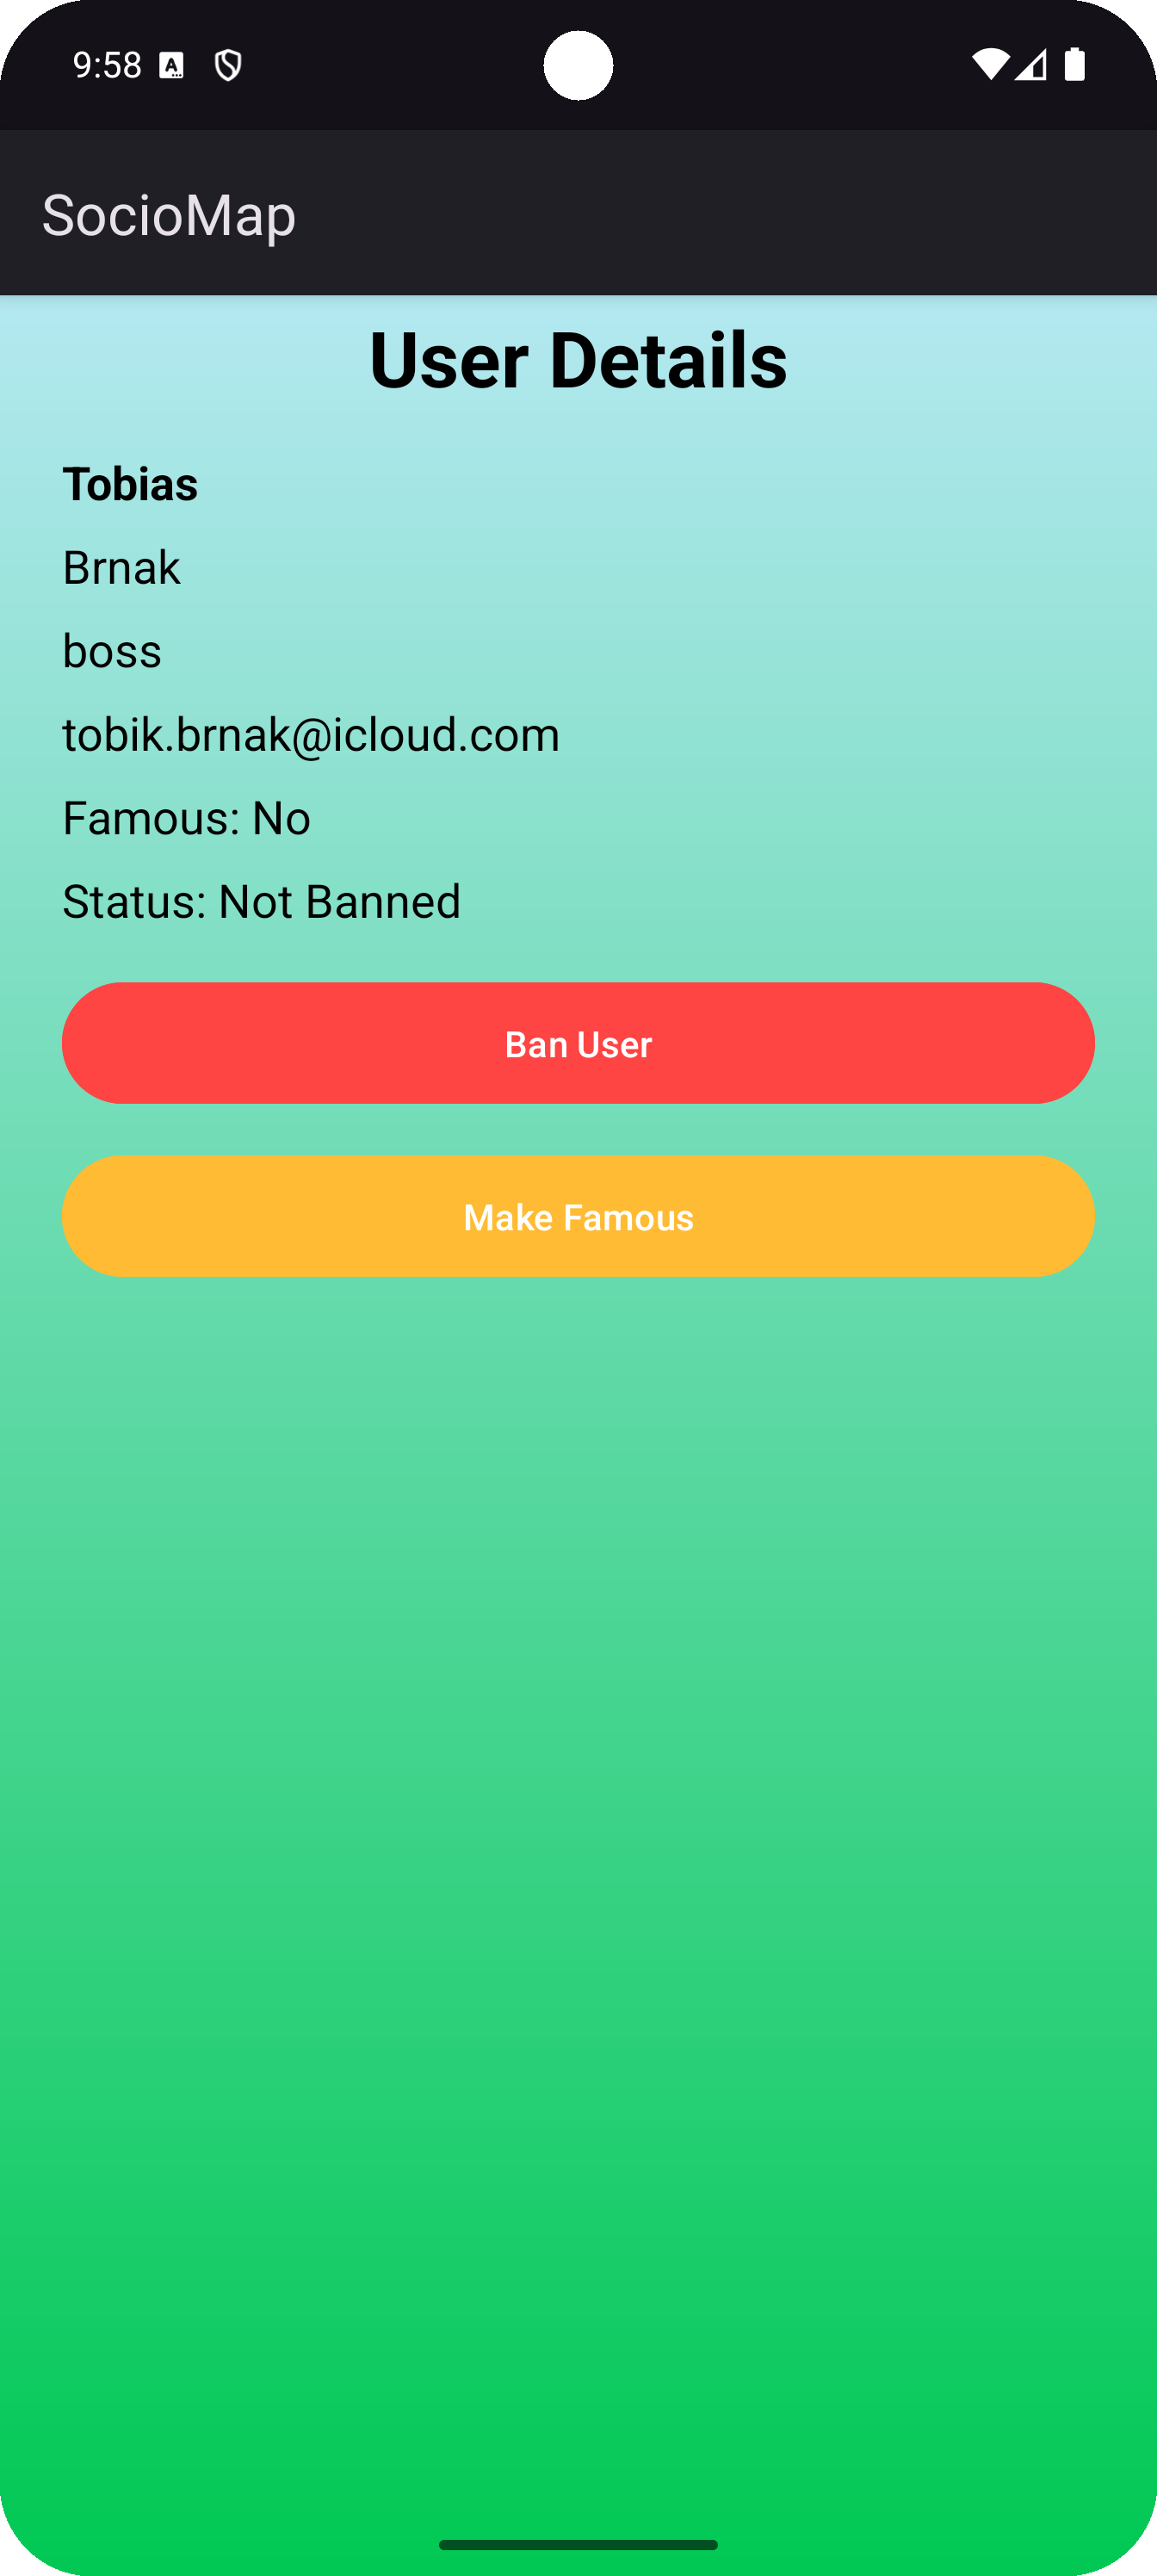
\includegraphics[height=11cm]{Images/AdminDetail.png}
    \caption{AdminUserDetails}
    \label{fig:Update-account}
\end{figure}








\subsection{Role a oprávnění uživatelů}

Aplikace SocioMapa rozlišuje tři základní typy uživatelů, kteří mají rozdílná oprávnění:

\begin{itemize}
    \item \textbf{Běžný uživatel} – může plně využívat funkcionality aplikace, jako je přidávání přátel, přihlašování se na události, vytváření vlastních událostí a filtrování záznamů v mapě. Má přístup pouze ke svým údajům a událostem.
    
    \item \textbf{Slavný uživatel (Famous)} – je vizuálně zvýrazněn pomocí speciálního designu. Na mapě se jeho události zobrazují pomocí odlišného stylu (např. korunka, výraznější barva markeru), což zvyšuje jejich viditelnost pro ostatní uživatele. 
    
    \item \textbf{Administrátor (Admin)} – má rozšířená oprávnění pro správu systému. Může:
    \begin{itemize}
        \item nastavovat status \texttt{isFamous} jiným uživatelům,
        \item blokovat účty pomocí příznaku \texttt{ban},
        \item zobrazovat podrobné informace o všech uživatelích.
    \end{itemize}
\end{itemize}

\begin{figure}
    \centering
    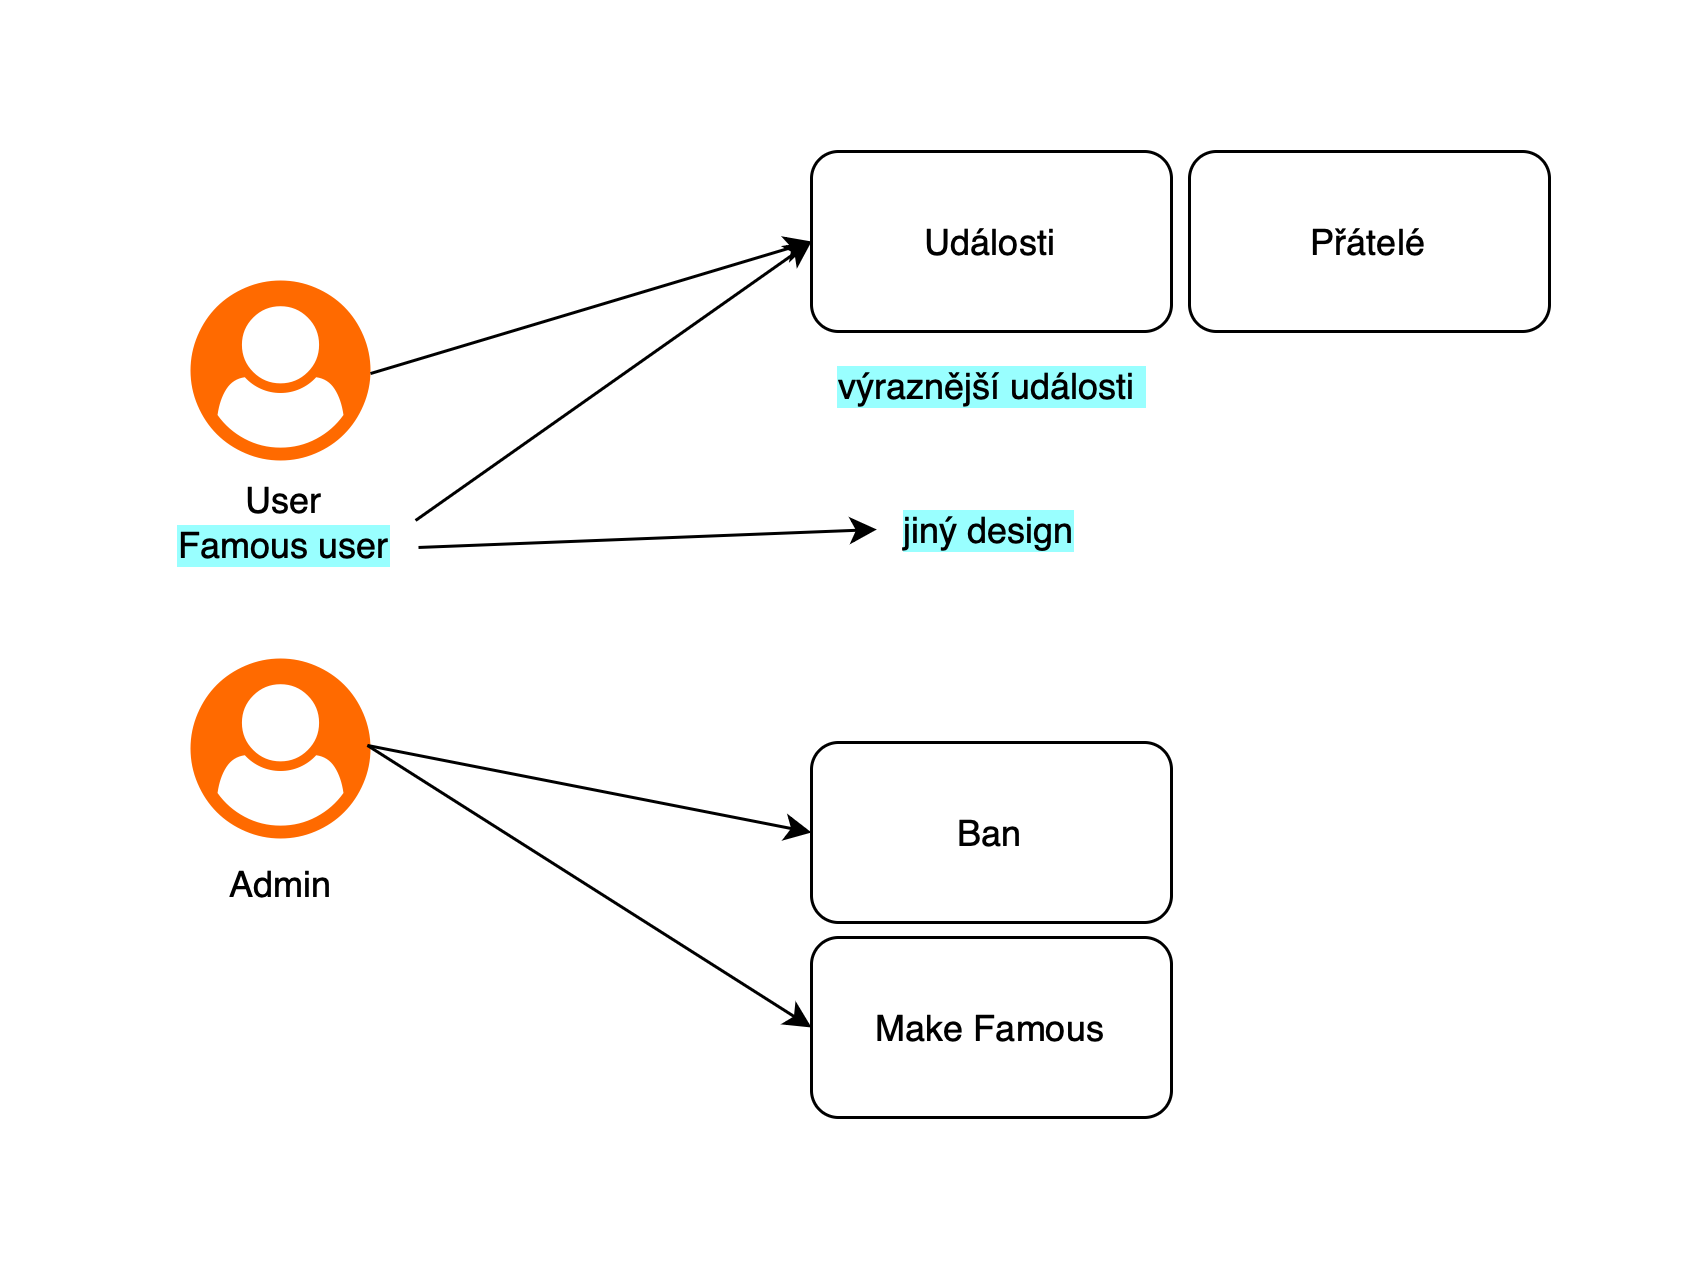
\includegraphics[width = \textwidth]{Images/User_relations.drawio.png}
    \caption{Role uživatele a jejich vztahy v systému}
    \label{fig:Update-account}
\end{figure}

Na obrázku je znázorněno, jak běžný uživatel a slavný uživatel interaguje s přáteli (sleduje je a vidí jejich aktivity) a s událostmi (vytváří je nebo se na ně přihlašuje). Admin uživatel smí interagovat s proměnnými jako jsou \textit{ban} a \textit{isFamous}.






